\documentclass[letterpaper, compsoc, conference]{IEEEtran}

\usepackage[ruled,vlined]{algorithm2e}
\usepackage{natbib}
\usepackage[cmex10]{amsmath}
\usepackage{array}
\usepackage[tight,footnotesize]{subfigure}
\usepackage[caption=false,font=footnotesize]{subfig}
\usepackage{url}
\usepackage{paralist}
\usepackage{tikz}
\usepackage{fancyhdr}
\usepackage{multirow}
\usetikzlibrary{snakes}
\usetikzlibrary{patterns}
\usetikzlibrary{circuits}
\usetikzlibrary{arrows,shapes.geometric,shapes.gates.logic.US,shapes.gates.logic.IEC,calc}

\begin{document}
\title{A Co-operative Parallel SAT Solver Based on Message Passing}

\author{
    \IEEEauthorblockN{Nayden Nedev}
    \IEEEauthorblockA{
        Department of Computer Science  \\
        Princeton University \\
        \textit{nnedev@cs.princeton.edu}
    } 
    \and \IEEEauthorblockN{Pramod Subramanyan}
    \IEEEauthorblockA{
        Department of Electrical Engineering \\
        Princeton University \\
        \textit{psubrama@princeton.edu}
    } 
}
\maketitle

\begin{abstract}
The Boolean Satisfiability Problem is a task with many practical applications
and is known to be NP-complete. Numerous different algorithms have been
proposed in the literature that effectively solve real-world instances of the
problem in a reasonable amount of time. 

With the advent of fast modern multiprocessor systems, new directions for
further improvement of the existing solutions arise. In this paper, we present a
parallel SAT solver algorithm based on conflict-driven clause sharing and
message passing. We evaluate our approach on the base of the popular sequential
MiniSAT solver and compare it with one of the most successful parallel solvers
- ManySAT. Our experiments show that the proposed approach achieve up to 164X
speedup. The average speedup when using four-core system is about 2X.

\end{abstract}

\section{Introduction}
The Boolean Satisfiability Problem, usually called just the SAT problem, 
is the task of finding an assignment of all variables of a boolean 
formula in such a way that the whole formula evaluates to a true value.

The SAT problem has been thoroughly investigated and understood during the last
several decades. A lot of work has been done in both investigating the
theoretical properties of the problem and its practical implications. It is the
first problem in computer science that has been classified as NP-complete
\cite{SATNP}. One of the reasons, because of which it is so important, is the
fact that a huge number of practical problems from various domains can be modelled
as instances of the SAT problem. Examples include problems from hardware design and
verification, artificial intelligence, graph theory, logistics and others. This 
resulted in extensive research of this problem and tremendous progress in finding 
efficient ways to solve SAT in a reasonable amount of time. Myriad sophisticated
algorithms~\cite{CHAFF, GRASP, MiniSat,PSATO,WalkSAT,DPLL,GRADSAT,ManySAT} have
appeared in the scientific literature and special competitions \cite{SATRace2008} 
have been organized to compare different ideas and implementations.

However, most of the modern SAT solvers are entirely sequential and do not try 
to introduce any kind of parallel computation in their algorithms. The advent 
of new powerful multiprocessor architectures brings new directions in which SAT 
solvers can be improved. The few existing parallel SAT solvers are based 
mainly on shared-memory techniques. In this work, we propose a new parallel 
algorithm that is based on message-passing.

The main contributions of the paper are:
\begin{itemize}
\item Elaborate and precise analysis of the weaknesses of previous attempts 
for parallization of SAT solvers.
\item A novel parallel SAT solving algorithm based on message passing.
\end{itemize}
The rest of this paper is organized as follows: we review related work in
Section \ref{sec:related}, describe our solution in more detail in Section
\ref{sec:strategy}, present experimental evaluation of our approach in Section
\ref{sec:results} and conclude in Section \ref{sec:finish}.

\section{Related Work}
\label{sec:related}

There are hundreds of different algorithms and their variations that have been
proposed for this problem. Basically, there are two main classes of modern
algorithms that are used to solve the SAT problem in practice: the
conflict-driven clause learning algorithm and the stochastic local search
algorithms. In the last years, parallel modifications of this approaches have
been proposed.

\subsection{Sequential Approaches}

This section provides a brief review of the advances in sequential SAT solvers.

\subsubsection{Davis-Putnam-Logemann-Loveland (DPLL)}

The DPLL algorithm, which is one of the first algorithmic techniques to solve
the problem of Boolean satisfiability is a complete search algorithm based on
back-tracking. DPLL uses the following heuristics before each recursive call:

\begin{itemize}
\item \textbf{Unit Propagation}: if a clause contains only one literal, it can
be only satisfied by giving such a value to the this literal that make it true. 

\item \textbf{Pure Literal Elimination}: if a variable occurs with only one
polarity in the whole formula, then it can be assigned with a value that
corresponds to this polarity.
\end{itemize}
These heuristics drastically reduce the search space.

\subsubsection{Conflict-Driven Clause Learning (CDCL)}

Conflict-driven clause learning (CDCL) was first proposed by the
GRASP~\cite{GRASP} solver. The key idea behind CDCL is that each time the
solver finds a part of search space that is unsatisfiable, it analyzes this
``conflict'' to learn a new clause. Keeping track of the \emph{learned clauses}
helps the solver not explore the same ``dead-ends'' over and over again.

\subsubsection{Modern Solvers: Chaff and MiniSat} 
Chaff~\cite{CHAFF} improves upon GRASP using two techniques.  The first is a
data structure that enables efficient traversal of the clause database when
performing unit propagation known as \textbf{two-literal watching}.

Two-literal watching maintains the invariant that two unassigned variables are
watched in every clause. In other words, when a literal is assigned to, it is
removed from the watchlist and replaced with an unwatched literal. When no
unwatched literal can be found, it means the clause is eligible for unit
propagation. The key advantage of two-literal watching is that it enables
efficient unit propagation without forcing the solver to traverse the entire
clause database.

The decision heuristic in a SAT solver determines which variable is to be
assigned to (``branched'' on) next.  \textbf{Variable State Independent
Decaying Sum (VSIDS)} was a decision heuristic instroduced by Chaff which tends
to make the SAT solver explore variables that were recently involved in
conflicts. VSIDS keeps track of an ``activity factor'' metric that is a measure
of the number of recent conflicts a variable has been involved in.  The
intuition behind the metric is that it improves ``search space locality'' as
variables recently involved in conflicts are more likely to be chosen by the
decision heuristic.  This in turn improves overall performance by helping the
solver ``close-out'' large regions of the search space.

One of the main improvements that MiniSat~\cite{MiniSat} made on Chaff was to
exploit input pre-processing and simplification. MiniSat has won a number of
the ``SAT-Race'' competitions and we use MiniSat version 2.2 as the baseline
for our work.

\subsubsection{Stochastic Local Search Algorithm}
Another popular approach is to apply local search in the space of possible
assignments such, i.e. iteratively improving the current solution of the
problem with respect to some heuristic until all the constraints are satisfied.
The most successful SAT solvers based on this technique are WalkSAT
\cite{WalkSAT} and GSAT \cite{GSAT}.

\subsection{Parallel Approaches}
In contrast to the work in sequential solvers, a relatively small number of 
high-performance parallel approaches have been proposed.

\indent The earliest attempt for a parallel solver is PSATO \cite{PSATO}. It tries
to parallelize the sequential SATO (SAtisfiability Testing Optimized) solver
\cite{SATO}. Both versions use trie to represent the boolean formula. The exploration
of the search space is organized in master/slave model.

\indent Most of the proposed approaches use DPLL as a basis. Jurkowiak et al.~\cite{Jurkowiak} propose a concurrent algorithm, based on DPLL, that uses work-stealing queues in order to balance the amount of work performed by different threads. Such load-balancing is needed, because of the irregular structure of the boolean formulas. 

\indent A lot of work has been done in attempt to improve Chaff. GrADSAT \cite{GRADSAT} is based on zChaff implementation and uses a large number of widely distributed commodity computational resources. Blochinger et al.~\cite{Blochinger} 
propose another shared-memory algorithm that uses distributed mobile agents to 
perform clause sharing. This method scales very well on computational grids.

\indent Usage of divide-and-conquer approaches is also common. At
 MiraXT~\cite{MiraXT} the threads share a database about all clauses, including the
learned ones. The synchronization on the writing to this database is based on
 locking. The read access does not need any synchronization. When a clause is learned 
by a thread, it is written to the shared database.

\indent pMiniSat~\cite{PMiniSat} is a parallelization of MiniSAT. It is a combination 
of many standard techniques such as divide-and-conquer, dynamic work-stealing using 
guiding paths, sharing short learn clauses, etc.

\indent The most notable recent parallel algorithm is ManySAT \citep{ManySAT}.
ManySAT uses a portfolio of complimentary sequential algorithms that are derived
from variations of the traditional DPLL algorithm. The basic idea is that each sequential algorithm broadcasts its learnt clauses to all the others.

\section{Parallelization Strategy}
\label{sec:strategy}

Our general strategy for parallelization is twofold. To a limited extent we use
divide and conquer strategy to ensure that the different processes are working
on different parts of the search space. However, processes co-operate with each
process by sharing learnt clauses with other processes. 

\subsection{Clause Sharing}

As the SAT solver explores the search space, it finds that certain regions of
the space are unsatisfiable. This occurs each time the solver runs into a
``conflict''. Modern solvers since GRASP~\cite{GRASP} \emph{analyze} each
conflict to learn clauses that ensure that ``dead-ends'' are never visited
again. In our solver, as in ManySAT~\cite{ManySAT}, clauses learnt by one
process are broadcast to all the other processes. This benefits speedup by
because clauses learned ensure that no other process visits that part 
of the search space again.

\subsubsection{What Clauses To Share}

One important design decision here is deciding which clauses are to be shared
with the other processes. As our results will show, sharing everything is not
feasible because the communication overhead outweighs any performance benefits
this may result in. Hamadi et al.~\cite{Hamadi} suggest sharing clauses which
contain no more than a certain number of literals. The intuition here is that
short clauses are more ``general'', while long clause are more ``specific''.
Hence, sharing short clauses is likely to be useful to processes regardless of
what part of the search space they are in. In contrast, long clauses are likely
to be useful to processes only if they are exploring the same part of the
search space. 

Note the SAT solver will most likely \textit{not} explore all parts of the
search space as this would simply take too long. Modern solvers are efficient
because they determine satisfiability by using heuristics to explore only
those parts of the search space that are likely to lead to a solution.

\subsubsection{Clause Sharing Based on Activity Factors}
Modern solvers since Chaff~\cite{CHAFF} maintain an ``activity factor'' for
each variable that is measure of the number of conflicts a variable has
recently been involved in. Variables with a high activity factor are chosen
by the decision heuristic when determining which part of the search to explore
next. 

Modern solvers chose to explore parts of the search space determined by
variables with a high activity factor.  If two processes are exploring
``nearby'' parts of the search space, they will likely have the same set of
variables with high activity factors. This suggests that activity factors may
be a useful measure to determine which clauses ought to be shared with which
variables. The challenge here is in communicating the activity factors from one
process to another without the communication overhead negating any performance
gains that may result from the clause sharing.

One of the goals of our project is to gain an understanding of what clauses
would be useful to share and design mechanisms for ``intelligent'' learned
clause sharing.  Activity factors are likely to be a useful metric in designing
such mechanisms.

\subsection{Decision Heuristic} 

The decision heuristic in a SAT solver determines which variable is to be
assigned to and ``branch'' on next. Modern SAT solvers use the activity factor
metric to determine which variable to branch on.

Our parallel SAT solver has to balance the competing interests of dividing the
search space among different processes while ensuring that they don't go too
``far away'' from each other. If the processes are exploring completely
independent parts of the search space, the learned clauses from one process
will likely not be useful to other processes. 

Our current decision heuristic balances these goals in the following way.  If
two variables have exactly the same activity factor, the heuristic biases
process $i$ towards variables $v_k$ such that $k~mod~i=0$. If two variables
have differing activity factors, the variable with higher activity is chosen.

\subsection{A Clustered Sharing Approach}

\begin{figure*}[htbp]
    \tikzstyle{box}=[rectangle,draw=black,thick,inner sep=2pt,text centered,
                     minimum height=8mm,minimum width=15mm]
    \tikzstyle{bigbox}=[rectangle,draw=black,thick,inner sep=2pt,text centered,
                        minimum height=8mm,minimum width=40mm, rounded corners=7]
    \begin{center}
    \begin{tikzpicture}
        \node[box] (c0) at (0,0) {\small{process 0}};
        \node[box] (c1) at (2,0) {\small{process 1}};
        \node[box] (c2) at (4,0) {\small{process 2}};
        \node[box] (c3) at (6,0) {\small{process 3}};
        \node[bigbox] (ic0) at (3,1.5) {\small{broadcast interconnect}};
        \draw[<->, thick] (c0.north) -- (ic0.210);
        \draw[<->, thick] (c1.north) -- (ic0.240);
        \draw[<->, thick] (c2.north) -- (ic0.300);
        \draw[<->, thick] (c3.north) -- (ic0.330);
    \end{tikzpicture}
    \end{center}
    \caption{Simple clause sharing broadcasts all learned clauses to every other process.}
    \label{fig:simple}
\end{figure*}

Figure \ref{fig:simple} shows the ``simple'' sharing approach. This is similar
to ManySAT and is the form of sharing implemented in the results shown. Each
process shares all learned clauses less than a certain maximum length with
every other process.

A different approach to clause sharing is shown in Figure \ref{fig:cluster}.
Here, the idea is that processes within the same cluster will share both long
and short clauses with each other. However, processes in different clusters
will only share short clauses with each other. The intuition here is that short
clauses are more general and hence likely to be useful to all processes while
the processes in a cluster are likely to be working on the same set of
variables and hence it makes sense to share longer and more specific clauses
with the rest of the cluster.

The clustered is yet to be fully implemented and results are not shown for it
in this preliminary report.
\begin{figure*}[htbp]
    \tikzstyle{box}=[rectangle,draw=black,thick,inner sep=2pt,text centered,
                     minimum height=8mm,minimum width=15mm]
    \tikzstyle{bigbox}=[rectangle,draw=black,thick,inner sep=2pt,text centered,
                        minimum height=8mm,minimum width=40mm, rounded corners=7]
    \begin{center}
    \begin{tikzpicture}
        \node[box] (c0) at (0,0) {\small{process 0}};
        \node[box] (c1) at (2,0) {\small{process 1}};
        \node[box] (c2) at (4,0) {\small{process 2}};
        \node[box] (c3) at (6,0) {\small{process 3}};
        \node[box] (c4) at (8,0) {\small{process 4}};
        \node[box] (c5) at (10,0) {\small{process 5}};
        \node[box] (c6) at (12,0) {\small{process 6}};
        \node[box] (c7) at (14,0) {\small{process 7}};
        \node[bigbox] (ic0) at (3,1.5) {\small{cluster interconnect}};
        \node[bigbox] (ic1) at (11,1.5) {\small{cluster interconnect}};
        \node[bigbox] (ic2) at (7,3.0) {\small{global interconnect}};

        \draw[<->, thick] (c0.north) -- (ic0.210);
        \draw[<->, thick] (c1.north) -- (ic0.240);
        \draw[<->, thick] (c2.north) -- (ic0.300);
        \draw[<->, thick] (c3.north) -- (ic0.330);
        
        \draw[<->, thick] (c4.north) -- (ic1.210);
        \draw[<->, thick] (c5.north) -- (ic1.240);
        \draw[<->, thick] (c6.north) -- (ic1.300);
        \draw[<->, thick] (c7.north) -- (ic1.330);

        \draw[<->, thick] (ic0.north) -- (ic2.240);
        \draw[<->, thick] (ic1.north) -- (ic2.300);
    \end{tikzpicture}
    \end{center}
    \caption{Clustered sharing shares long and short clauses with the local cluster 
             while broadcasting only short clauses to all the other processes.}
    \label{fig:cluster}
 \end{figure*}

\section{Results}
\label{sec:results}

The section describes our preliminary results with the simple clause sharing
technique described earlier. The results shown in Section \ref{sec:speedup}
share clauses with 16 literals or fewer with all the other cores. Section
\ref{sec:sharing effects} investigates the impact of sharing shorter
and longer clauses.

\subsection{Methodology}
Our benchmark problems are taken from SAT-Race 2008~\cite{SATRace2008}. We
executed all 100 problems used in the competition using the sequential SAT
solver MiniSat 2.2 with a time limit of 5 minutes.\footnote{MiniSat 2.1 was the
fastest solver in SAT-Race 2008} Among these 100 problems, we chose to
experiment with a subset of 25 problems that took MiniSat 2.2 between 40s and
200s to execute. Our intention in choosing this subset was to choose a small
number of problems that we could execute relatively quickly and often while
simultaneously ensuring that we avoid those that finished in a few seconds.  We
intend to present full results in the standard SAT-Race format (time limit of
15 minutes) for the final submission of this report.

Fourteen among the chosen 25 problems are satisfiable while the remaining
eleven are unsatisfiable. The comparison with ManySAT uses ManySAT version 2.0
obtained from~\cite{ManySATWeb}.  The default command-line and default
parameter settings were used when executing ManySAT.


Experiments were performed on an 8-core Intel\textregistered
~Xeon\textregistered ~E31230 CPU clocked at 3.20GHz with 32 GB of RAM (machine 1)
and a 24-core Intel\textregistered~Xeon ~E5645 CPU clocked at 2.40 GHz with
132GB of RAM (machine 2). 

\subsection{Speedup}
\label{sec:speedup}

\begin{table*}[htbp]
    \begin{center}
    \begin{tabular}{|l|c|c|c|c|c|c|c|c|}
        \hline
        {\textbf{SAT Benchmark}} & \multicolumn{4}{c|}{\bf ManySAT 2.0} & \multicolumn{4}{c|}{\bf MPI-based Parallel Solver} \\
        \hline
        & $n=1$ & $n=2$ & $n=4$ & $n=8$ & $n=1$ & $n=2$ & $n=4$ & $n=8$ \\
        \hline
        ibm-2004-29-k25                    &       1.0 &  1.5 &  2.8 &  2.4 &  1.0 &  1.1 &  2.5 &  2.9 \\
        ibm-2004-1\_11-k80                 &       1.0 &  0.6 &  0.9 &  0.8 &  1.0 &  0.7 &  0.8 &  1.1 \\
        ibm-2002-20r-k75                   &       1.0 &  1.3 &  1.9 &  0.8 &  1.0 &  1.1 &  2.6 &  1.7 \\
        simon-s02b-r4b1k1.2                &       1.0 &  3.4 &  4.7 & 47.6 &  1.0 & 25.7 & 22.6 &  3.3 \\
        velev-npe-1.0-9dlx-b71             &       1.0 &  0.4 &  1.0 &  0.6 &  1.0 &  3.7 &  1.7 &  1.6 \\
        schup-l2s-motst-2-k315             &       1.0 &  0.8 &  1.0 &  1.2 &  1.0 &  0.5 &  1.1 &  0.8 \\
        goldb-heqc-alu4mul                 &       1.0 &  2.1 &  2.6 &  2.7 &  1.0 &  1.9 &  3.3 &  3.0 \\
        jarvi-eq-atree-9                   &       1.1 &  1.6 &  2.6 &  6.9 &  1.0 &  1.2 &  2.5 &  2.0 \\
        ibm-2002-22r-k80                   &       1.0 &  0.7 &  2.4 &  0.9 &  1.0 &  0.5 &  1.0 &  1.8 \\
        simon-s03-fifo8-400                &       1.0 &  1.7 &  1.7 &  1.8 &  1.0 &  1.8 &  1.9 &  2.2 \\
        ibm-2002-24r3-k100                 &       1.0 &  2.0 &  2.2 &  2.5 &  1.0 &  1.8 &  2.3 &  3.0 \\
        mizh-sha0-36-4                     &       1.0 &  2.4 &  3.9 &  3.2 &  1.0 &  0.2 &  0.8 &  0.6 \\
        manol-pipe-f7nidw                  &       1.0 &  1.8 &  2.4 &  1.9 &  1.0 &  1.6 &  2.3 &  2.4 \\
        manol-pipe-c6bidw\_i               &       1.0 &  1.1 &  1.8 &  1.6 &  1.0 &  1.5 &  1.6 &  2.0 \\
        mizh-md5-47-3                      &       1.0 &  0.6 &  1.3 &  1.7 &  1.0 &  1.4 &  2.3 &  5.6 \\
        ibm-2004-23-k80                    &       1.0 &  0.9 &  0.7 &  1.0 &  1.0 &  0.7 &  1.1 &  3.5 \\
        mizh-md5-48-2                      &       1.0 &  0.2 &  0.3 &  0.9 &  1.0 &  1.4 &  2.2 &  5.9 \\
        ibm-2002-22r-k75                   &       1.0 &  1.0 &  1.8 &  1.8 &  1.0 &  1.8 &  1.9 &  2.0 \\
        manol-pipe-g10nid                  &       1.0 &  1.4 &  1.8 &  1.5 &  1.0 &  1.3 &  1.8 &  1.6 \\
        fuhs-aprove-16                     &       1.0 &  0.8 &  1.3 &  1.4 &  1.0 &  1.0 &  1.7 &  1.7 \\
        post-c32s-col400-16                &       1.0 &  1.2 &  1.7 &  2.2 &  1.0 &  1.5 &  2.1 &  2.3 \\
        anbul-dated-5-15-u                 &       1.0 &  1.9 &  2.5 &  2.3 &  1.0 &  2.0 &  2.0 &  1.7 \\
        mizh-sha0-35-4                     &       1.0 &  3.3 &  2.3 &  3.1 &  1.0 &  5.9 &  1.6 &  9.0 \\
        ibm-2004-29-k55                    &       1.0 & 14.1 & 20.0 & 15.2 &  1.0 & 21.5 &164.3 & 59.2 \\
        mizh-sha0-36-1                     &       1.0 &  0.6 &  1.0 &  3.9 &  1.0 &  0.6 & 11.2 & 14.6 \\
        \hline
        \textbf{total}                     &       1.0 &  1.0 &  1.5 &  1.8 &  1.0 &  1.1 &  2.0 &  2.3 \\
        \hline
    \end{tabular}
    \end{center}
    \caption{Speedup of parallel SAT solvers on machine 1 as $n$ (number of
    cores) is varied. Speedup is computed using MiniSat 2.2 as the baseline. }
    \label{tab:speedup}
\end{table*}

Table \ref{tab:speedup} shows the speedup of the ManySAT 2.0 and our
implementation for the 25 selected benchmarks. Speedups are shown for 1, 2, 4
and 8 cores running on machine 1.  Our implementation shows significant speedup
($>2X$) when using 4 cores and slightly more than that for 8 cores. Since
learnt clauses are broadcast to all the other cores, it would seem that
communication overheard for 8 cores outweighs the sharing benefit. 

We note that super-linear speedups are possible and observed in a number of
benchmarks.  Since SAT-solving is essentially a heuristic search, combining
information from multiple processes can help the solver ``close out'' large
regions of the search space much faster than would have been possible with a
sequential search. It is not necessary that the sizes of ``closed out'' regions
is linearly proportional to the number of cores. We also not that co-operation
can be detrimental because of the interaction between the shared clauses and
the decision heuristic.  This can can result in the solver ``wasting time'' by
exploring parts of the search space that do not contain the solution.

\begin{figure}[htbp]
    \begin{center}
        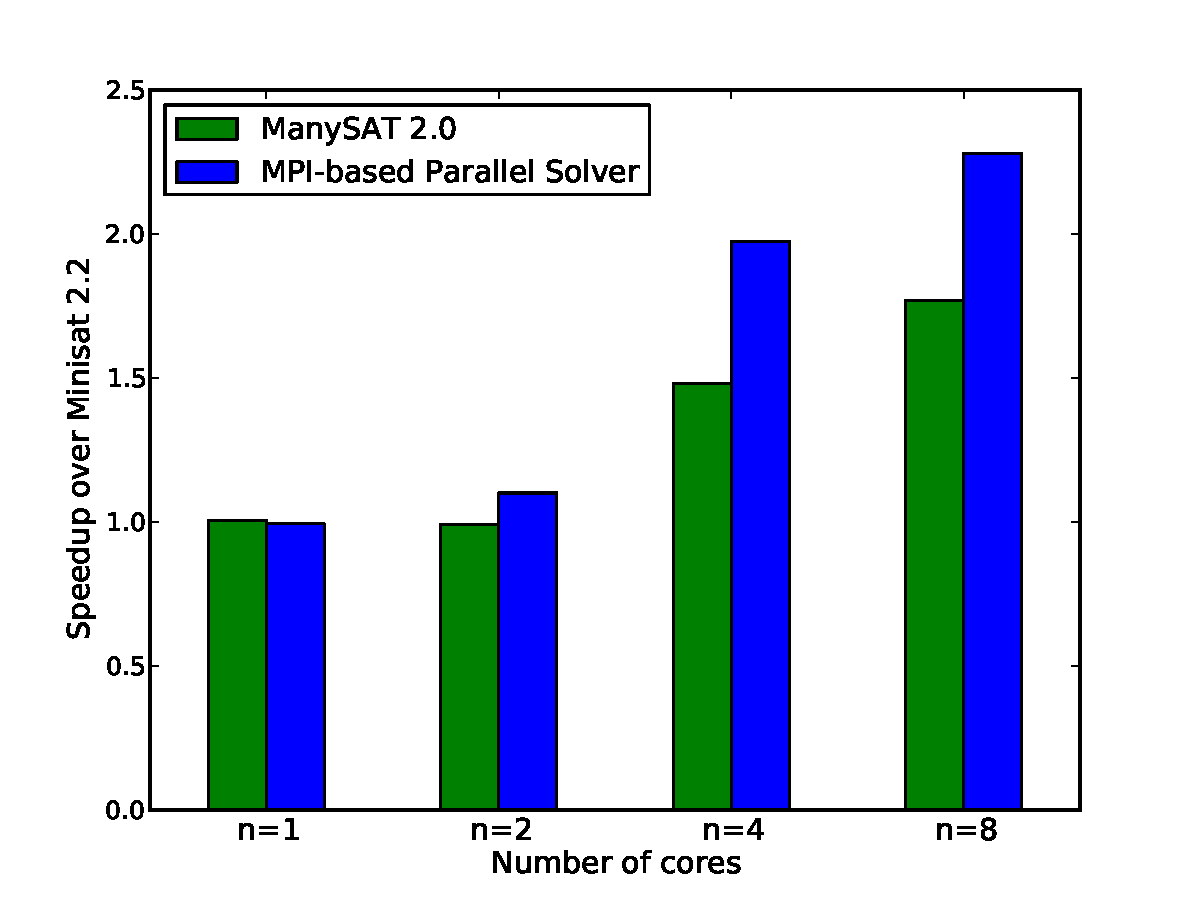
\includegraphics[width=\columnwidth]{images/speedup1.pdf}
        \caption{Overall Execution Speedup.}
        \label{fig:speedup}
    \end{center}
\end{figure}

Figure \ref{fig:speedup} presents the \emph{overall execution speedup} for the
problems shown in Table \ref{tab:speedup}. The overall speedup measured here is
speedup compared to MiniSat 2.2 baseline for the time taken to solve all 25
problems by the two parallel solvers. It can be seen that the MPI-based
parallel solver gets only slightly faster when going from 1 to 2 cores. Going
from 2 to 4 cores produces significant speedup but speedup is already tapering
off at 8 cores. The MPI-based parallel solver out-performs ManySAT 2.0 by a
small amount for both 4 and 8 cores.

\subsection{Scalability}
\label{sec:scalability}

\begin{table*}[htbp]
    \begin{center}
    \begin{tabular}{|l|c|c|c|c|c|c|}
        \hline
        {\textbf{SAT Benchmark}} & \multicolumn{6}{c|}{\textbf{Number of Cores}} \\
        \hline
        & $n=4$ & $n=8$ & $n=12$ & $n=16$ & $n=20$ & $n=24$ \\
        \hline
      ibm-2004-29-k25.cnf.gz &                   3.4 &  5.3 &  6.5 &  6.9 &  6.3 &  6.2 \\
      ibm-2004-1\_11-k80.cnf.gz &                1.8 &  1.7 &  2.3 &  2.8 &  2.2 &  2.7 \\
      ibm-2002-20r-k75.cnf.gz &                  1.4 &  2.7 &  2.5 &  2.5 &  1.9 &  2.2 \\
      simon-s02b-r4b1k1.2.cnf.gz &               6.6 &  3.4 &  6.3 &  7.0 & 20.4 & 13.9 \\
      velev-npe-1.0-9dlx-b71.cnf.gz &            2.1 &  3.5 &  2.8 &  2.3 &  0.6 &  0.8 \\
      schup-l2s-motst-2-k315.cnf.gz &            1.1 &  1.7 &  1.4 &  2.0 &  1.7 &  1.7 \\
      goldb-heqc-alu4mul.cnf.gz &                3.6 &  5.8 &  6.2 &  6.0 &  6.4 &  6.0 \\
      ibm-2002-22r-k80.cnf.gz &                  1.2 &  1.7 &  2.1 &  2.0 &  1.7 &  1.7 \\
      simon-s03-fifo8-400.cnf.gz &               2.2 &  3.1 &  3.1 &  3.4 &  3.2 &  3.4 \\
      ibm-2002-24r3-k100.cnf.gz &                3.6 &  4.3 &  4.2 &  4.4 &  5.4 &  5.0 \\
      manol-pipe-f7nidw.cnf.gz &                 3.1 &  4.6 &  4.6 &  4.2 &  3.5 &  3.4 \\
      manol-pipe-c6bidw\_i.cnf.gz &              2.5 &  3.2 &  3.5 &  3.5 &  3.4 &  3.2 \\
      ibm-2004-23-k80.cnf.gz &                   0.7 &  1.3 &  1.6 &  2.0 &  1.4 &  2.5 \\
      ibm-2002-22r-k75.cnf.gz &                  2.6 &  2.5 &  4.3 &  4.3 &  4.0 &  3.5 \\
      manol-pipe-g10nid.cnf.gz &                 2.3 &  2.5 &  2.7 &  2.4 &  2.5 &  2.3 \\
      fuhs-aprove-16.cnf.gz &                    1.5 &  2.3 &  2.4 &  2.4 &  2.7 &  3.0 \\
      post-c32s-col400-16.cnf.gz   &             2.5 &  2.9 &  3.4 &  3.3 &  3.1 &  2.7 \\
      anbul-dated-5-15-u.cnf.gz &                2.6 &  4.3 &  4.5 &  4.1 &  5.0 &  3.8 \\
      mizh-sha0-35-4.cnf.gz &                    0.7 &  2.8 & 13.0 & 13.1 &  7.8 &  2.2 \\
      ibm-2004-29-k55.cnf.gz &                   8.3 & 29.6 & 23.3 & 24.6 & 25.6 & 21.2 \\
      \hline
      \textbf{total}  &                          1.8 &  3.0 &  3.5 &  3.6 &  3.0 &  2.9 \\
      \hline
    \end{tabular}
    \end{center}
    \caption{Speedup of MPI-based Parallel Solver on machine 2. Minisat 2.2 is again
    used as the baseline.}
    \label{tab:scalability}
\end{table*}

To study the scalability of the MPI-based solver we used machine 2 and measured
speedup over the MiniSAT 2.2 baseline for 4, 8, 12, 16, 20 and 24 cores. We
found that ManySAT2.0 was crashing on some instances when running on more than
8 cores, so we do not present the results for ManySAT in this table. We also
found that some of the 25 instances timed out\footnote{The timeout was set to
1000 seconds.} so results for these instances are not shown if any one of the
experiments timed out. Leaving out these instances left us with the 20
benchmarks shown in Table \ref{tab:scalability}. 

We see from Table \ref{tab:scalability} that some performance improvements are
seen up to 16 cores but there is a slowdown when running the program with 20
and 24 cores. This suggests that beyond 16 cores, the overhead of communication
and the divide-and-conquer approach outweighs the benefits of clause sharing.

\subsection{Effect of Clause Sharing}
\label{sec:sharing effects}

\begin{figure}[htbp]
    \begin{center}
        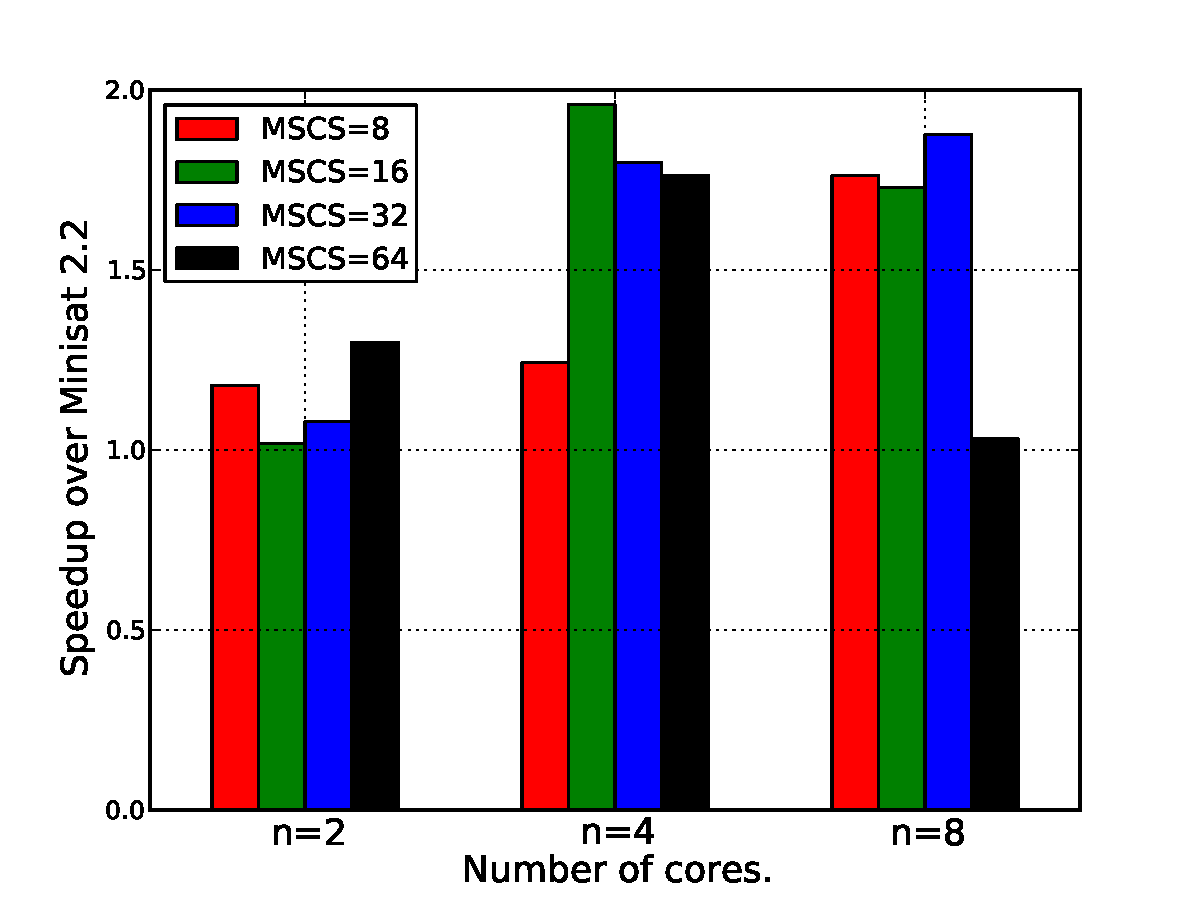
\includegraphics[width=\columnwidth]{images/mcs.pdf}
        \caption{Effect of maximum shared clause size (MSCS) (machine 1).}
        \label{fig:mscs}
    \end{center}
\end{figure}

Figure \ref{fig:mscs} shows the effect of maximum size of shared clauses on the
speedup for machine 1. Note these results are slightly different from those
shown in Figure \ref{fig:speedup} because of noise in the timing measurements.
Although the trends are somewhat hard to interpret because of the noise, some
observations that can be made are the following.

\begin{enumerate}

\item When executing with only 2 cores, sharing as many clauses as possible
(i.e., up to maximum sharing clause size (MSCS) of 64) is beneficial.

\item When executing with four cores, the best performance is achieved when
MSCS=16. This number corresponds to the results shown in the previous
subsection.

\item When executing with either cores, sharing less (MSCS=8) seems to be the
best although there is an abberant data point for MSCS=32.
      
\end{enumerate}

\begin{figure}[htbp]
  \begin{center}
    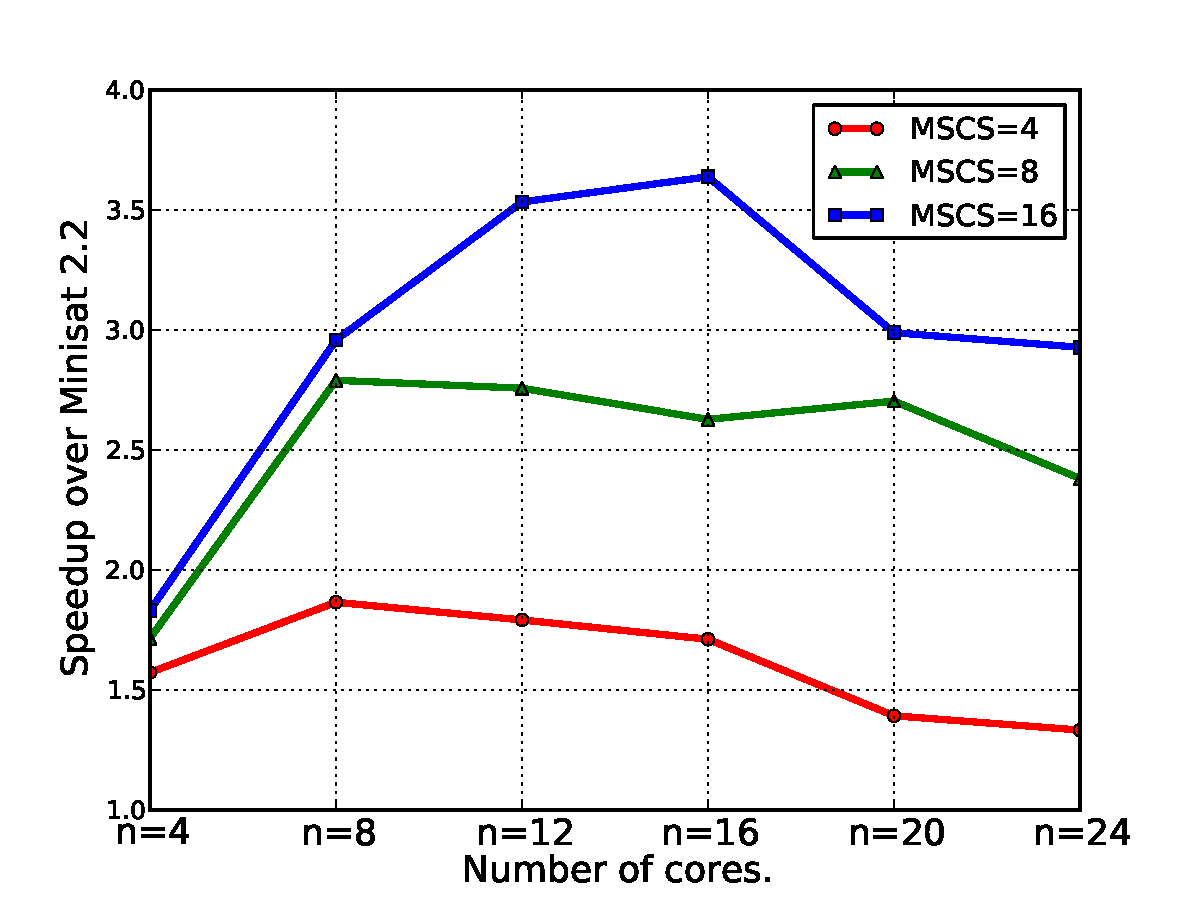
\includegraphics[width=\columnwidth]{images/mcs2.pdf}
    \caption{Effect of maximum shared clause size (MSCS) (machine 2).}
    \label{fig:mscs2}
  \end{center}
\end{figure}

Figure \ref{fig:mscs2} shows the impact of the maximum shared clause size on
machine 2. This graph makes it very clear that sharing fewer clauses is
\emph{not} beneficial for scalability because although this lesses the overhead
of communication, it also results in processes co-operating less, hurting
speedup. We also see that MSCS=16 is not beneficial for anything more than 16
cores likely because of the overhead of all-to-all broadcasting of learned
clauses.

\subsection{Measuring Impact of Clause Sharing}

\begin{figure*}[htbp]
    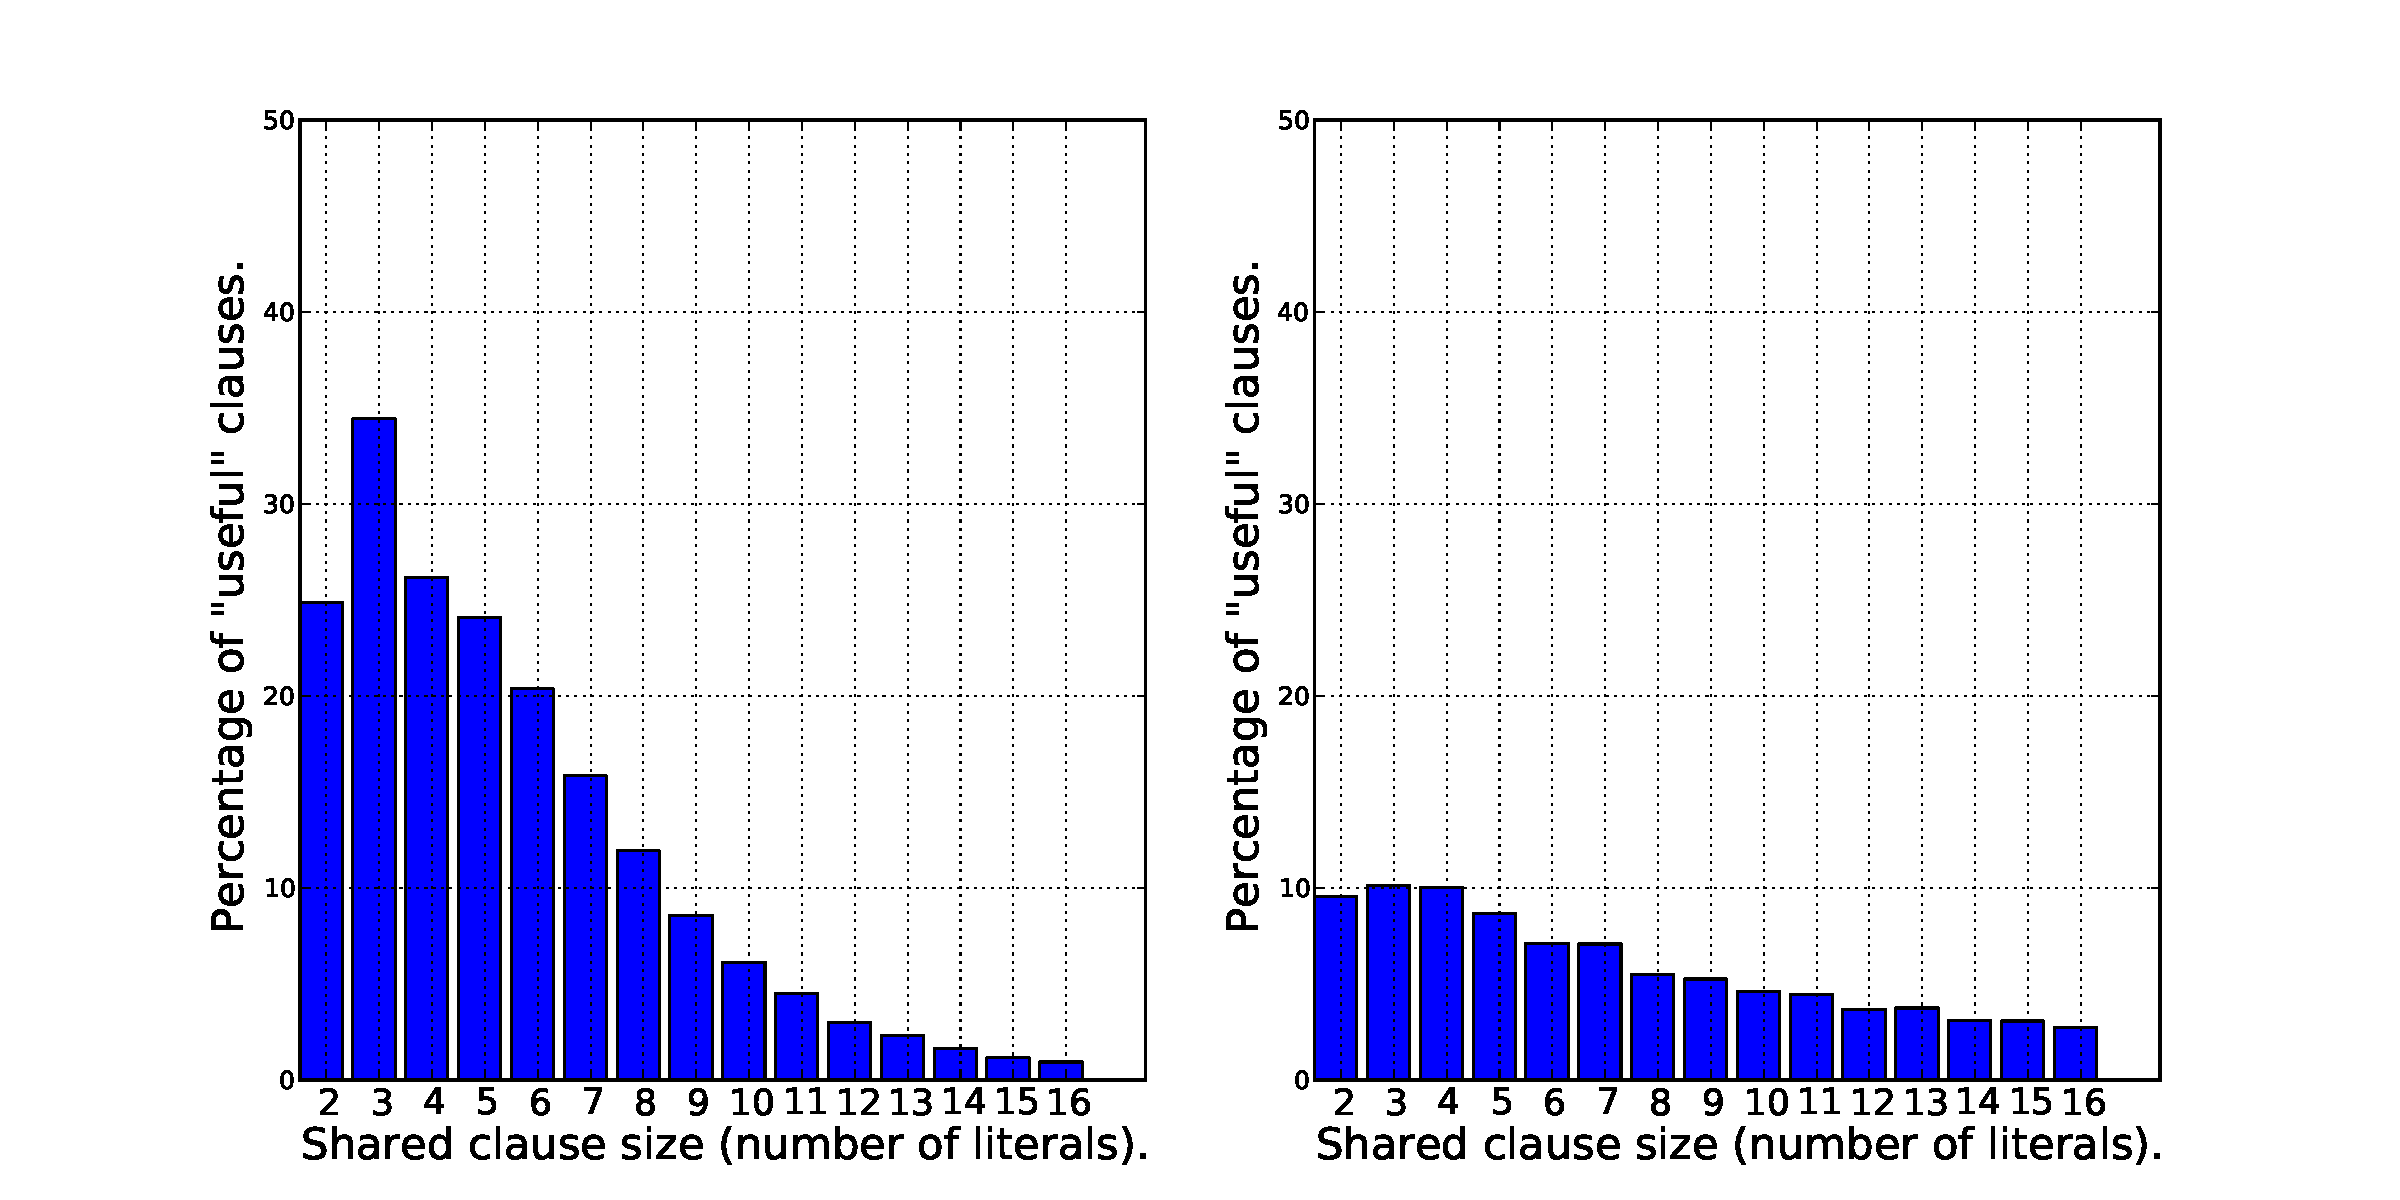
\includegraphics[width=2\columnwidth]{images/useful.pdf}
    \caption{Distribution of useful and useless clauses as a percentage of total
    imported clauses vs. clause size for (left) mizh-sha0-36-4 on 2 cores and
    (right) ibm-2004-29-k55 on 4 cores.}
    \label{fig:useful}
\end{figure*}


To quantify the impact of clause sharing, we instrumented the solver to keep
track of learnt clauses that arrived from another process and then count the
number of such clauses that were involved in at least one conflict.  We refer
to a learned class obtained from another process as an ``imported''
clause.\footnote{The term ``imported'' clause is borrowed from the ManySAT
codebase.} An imported clause that subsequently causes a conflict is called a
``useful'' clause. Clearly, imported clauses that never get involved in a
conflict are undesireable because they simply contribute to the communication
overhead without aiding any of the computation.

Figure \ref{fig:useful} shows the percentage of clauses and the distribution of
their sizes for two benchmarks. The graph on the left is for
\textit{mizh-sha0-36-4} executed on two cores which has poor speedup. The graph
on the right is for \textit{ibm-2004-29-k55} executing on 4 cores. This has
good speedup. \textit{mizh-sha0-36-4} shares a lot of useful short clauses but
very few useful long clauses. For \textit{ibm-2004-29-k55}, we see that the
distribution of the length of useful clauses is more uniform. This pattern was
observed in a few other benchmarks with good speedup, which suggests that
successfully sharing useful long clauses is important for performance. One
intuitive explanation for this could be that if the processes are sharing
useful long clauses, it means they are co-operating to a greater extent than if
they are just sharing useful short clauses. 

{The lesson here is that the parallel processes in the solver must co-operate
as much possible while making sure they don't end up doing redundant work to
get good performance.} Simply exploring different parts of the search space is
unlikely to result in useful co-operation/good performance. The other big
takeaway from the figure is that the majority of clauses are actually useless,
which suggests that there is potential here to improve scalability by the
design of intelligent heuristics that share only a subset of learned clauses.

\subsection{Clustered Sharing Results}
\begin{figure}[htbp]
  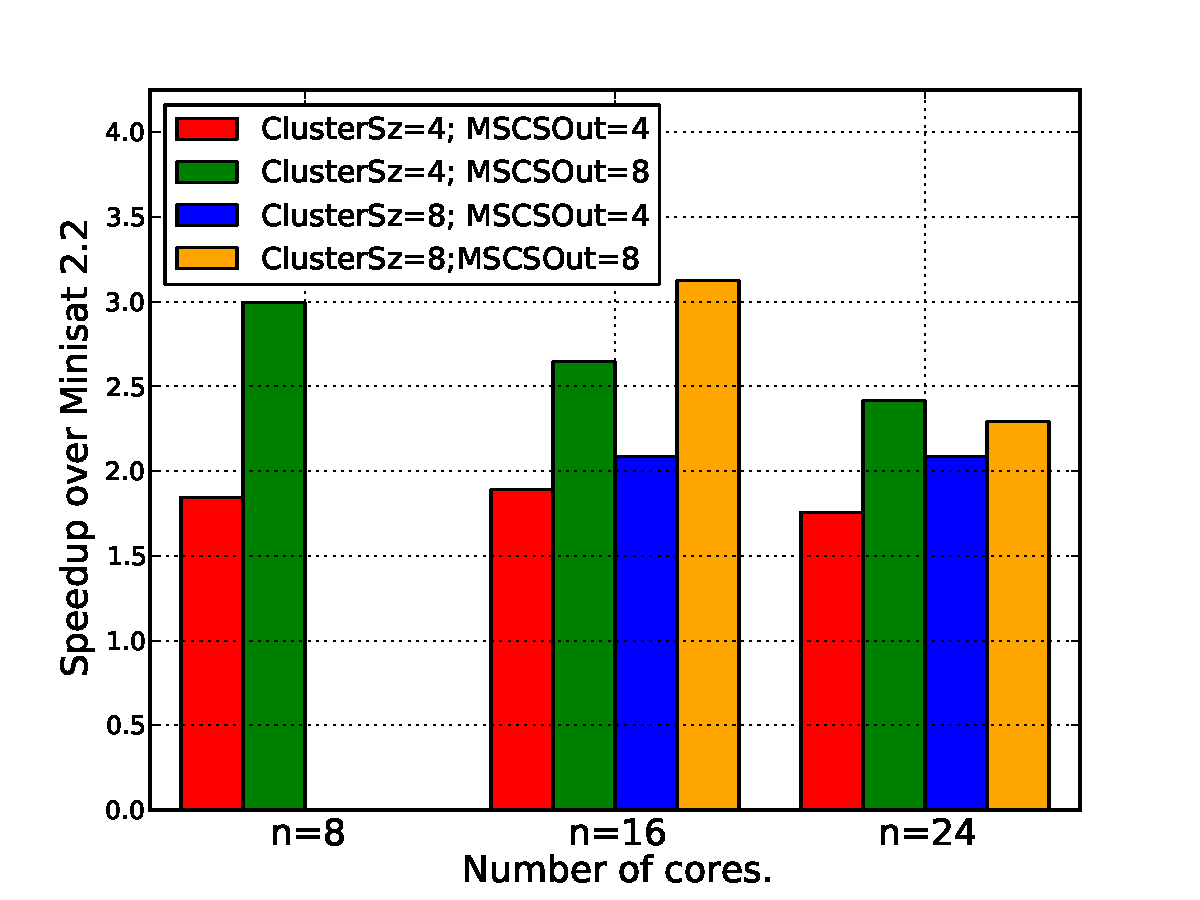
\includegraphics[width=\columnwidth]{images/cluster.pdf}
  \caption{Results of solver with clustered sharing (machine 2).}
  \label{fig:cluster}
\end{figure}

Figure \ref{fig:cluster} shows the impact of ``clustered clause sharing''. In
this experiment, ``clusters'' are formed containing either 4 or 8 cores. Each
core exports all learned claused with 16 or fewer literals to all the cores in
its cluster. However, it only exports clauses with fewer than either 4 or 8
(labeled MCSCOut) to the cores outside the cluster. In other words, there is
more communication within the cores in a cluster than between cores in different
clusters.

The results show that MSCSOut=8 outperforms MSCSOut=4, which again supports our
hypothesis that effective co-operation is essential for good performance. We
also note that all the clustered configurations are outperformed by the default
configuration that uses all-to-all broadcast. 


\subsection{Approximate comparison of activity factors}
The default divide and conquer algorithm biases invidual cores towards certain
variables only when the activity factors for the variables are exactly the same.

\begin{figure}[htbp]
  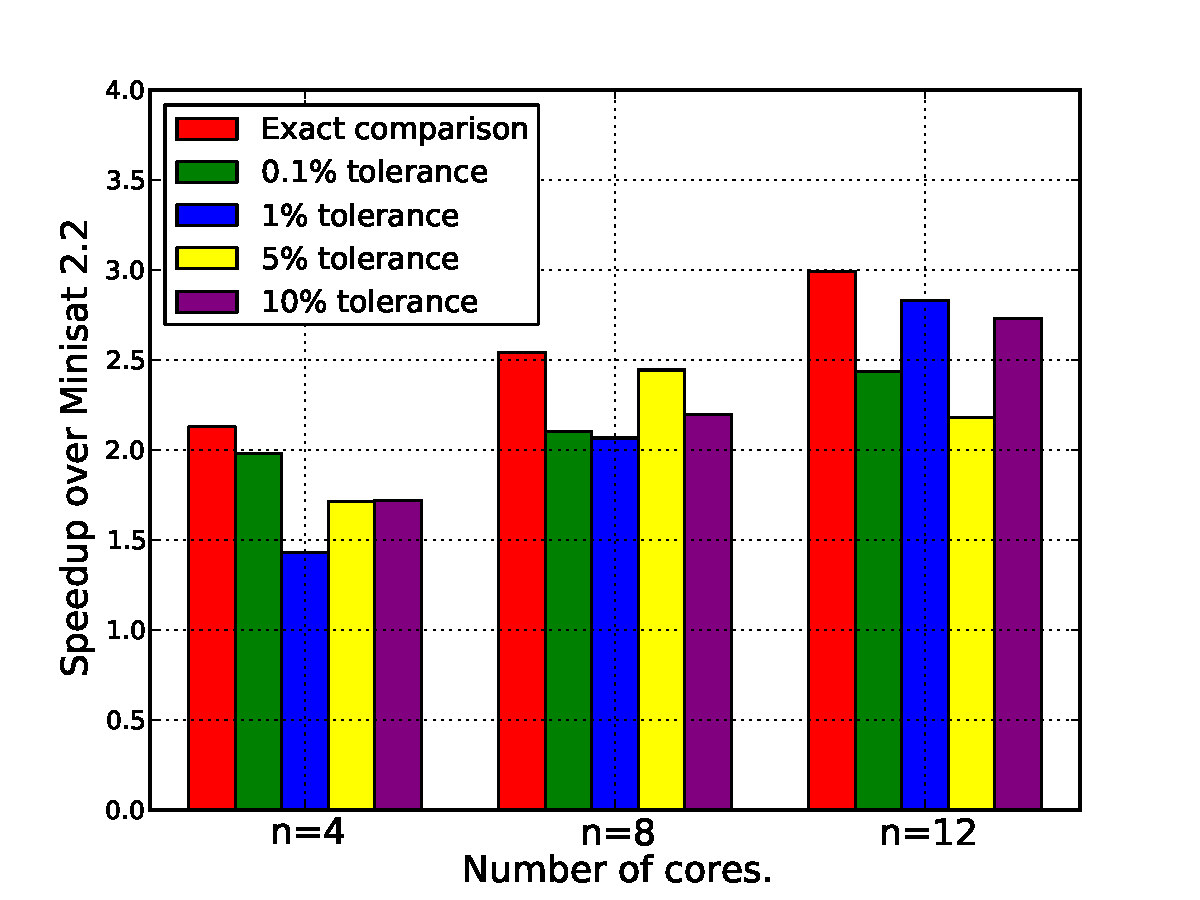
\includegraphics[width=\columnwidth]{images/aff.pdf}
  \caption{Impact of approximate comparison of activity factors (machine 2).}
  \label{fig:aff}
\end{figure}

Figure \ref{fig:aff} shows the impact of approximate comparison of the activity
factors instead of exact comparison when choosing to bias the activity heuristic.
We study tolerances range from $0.1\%$ to $10\%$ and find that exact comparison
is actually the best option!

\subsection{Impact of the Base Restart Interval}

\begin{figure}[htbp]
  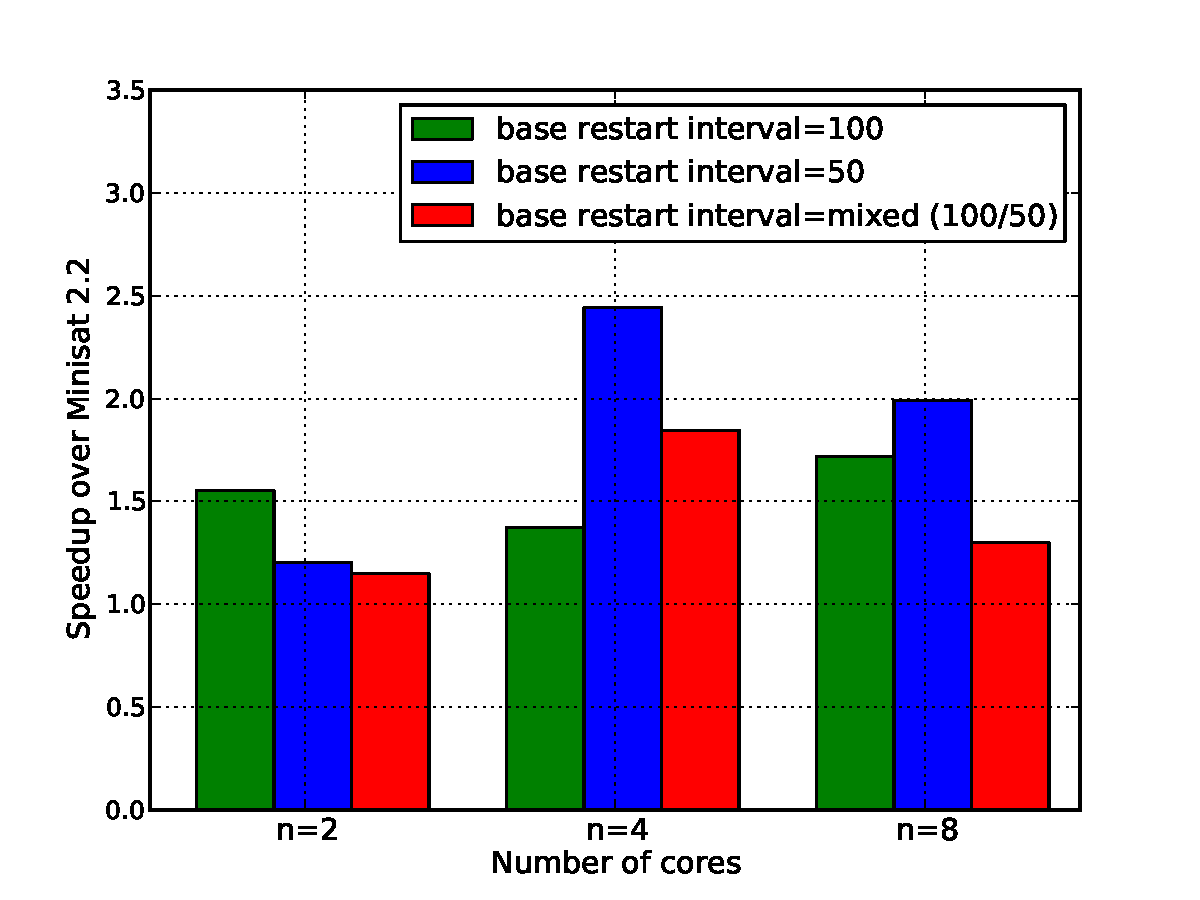
\includegraphics[width=\columnwidth]{images/restart_speedup1.pdf}
  \caption{Impact of Base Restart Interval (machine 1)}
  \label{fig:restart}
\end{figure}

Recent work \cite{HuangRestart2007} has suggested that the restart policy in
modern SAT-solver is a potential source of significant performance improvement.
MiniSAT uses the Luby sequence of restarts~\cite{Luby93optimalspeedup}
which means the solver restarts its search after $1X$, $1X$, $2X$, $1X$, $1X$,
$2X$, $4X$, $1X$, $1X$, $2X$, $1X$, $1X$, $2X$, $4X$, $8X$, $\dots$ conflicts
where $X$ is the base restart interval. 

Figure \ref{fig:restart} shows the effect of reducing the base restart interval
from the default value of $100$ conflicts to $50$ conflicts.\footnote{Note the
results cannot be compared directly with those shown previously because in this
experiment the solver was been instrumented to gather sharing statistics,
possibly making it a little slower.} It is evident that a smaller base restart
interval improves performance, which makes intuitive sense because the parallel
solver ``learns faster'' than a sequential solver. 

The red bar shows the performance of using a ``mixed'' base restart interval.
Half the processes use a restart interval of 100 conflicts while the others use a
restart interval of 50 conflicts. The intuition here was that mixed restart
intervals would desynchronize the processes which might help performance by
improving solver diversity. However, it appears this hurts performance more
than it helps because of the loss of co-operation among processes.

\section{Conclusion}
\label{sec:finish}

We presented a new technique for parallelization of SAT solvers based
on message passing. Our algorithm uses the conflict-driven clause learning 
and the popular MiniSAT as an implementation basis. Our results show that 
message passing is a promising approach for parallelizing this kind of 
applications and has some advantages over shared memory. Moreover, it is
competitive with modern award-winning high-performance implementations such as ManySAT. \\
\indent However, there are still many questions that have to be answered. Different 
communication patterns in combination with a variety of heuristics and also the mentioned clustered approach are going to be further explored.

\section*{Acknowledgements}

We would like to thank Professor David Wentzlaff and Professor Sharad Malik for
sharing their suggestions and ideas with us.

\bibliographystyle{plain}
\bibliography{report}
\end{document}
